\documentclass[12pt, letter]{article}
\usepackage[utf8]{inputenc}
\usepackage{amsfonts,amssymb,amsthm,amsmath}
\usepackage[margin=1in]{geometry}
\usepackage[dvipsnames]{xcolor}
\usepackage{pgf}
\usepackage{graphicx}
\usepackage{hyperref}
\usepackage{tikz}
\usetikzlibrary{positioning}
\usepackage[bottom]{footmisc}
\usepackage{float}
\usepackage{fancyhdr}
\documentclass{article}
\usepackage[utf8]{inputenc}
\usepackage{graphicx}
\usepackage{hyperref}


% \pagestyle{fancy}
% \fancyhf{}
% \lhead{\leftmark}
% \cfoot{\thepage}

\title{\textbf{MTL782 Data Mining Assignment Subsmission}}
\author{Nitin Gautam\footnote{hes207035@hss.iitd.ac.in} \hspace{+3mm} \\Submitted to Prof. Bhawani Shankar Panda \footnote{as part of the course requirement in MTL 782 Data Mining}}
\date{March 27th, 2022}

\maketitle
\begin{Note}
\begin{itemize}
    \item The project is solely done by me, as unable to find group member who were interested in dataset (Pregnant women Risk stratification in developing countries), which is area of interest in development economics. Similar studies are carried out using NFHS survey dataset in India (National Family Health survey - 5)\\ 
    \item Jupyter notebook python Code is appended in appendix in this report for both Question 1 and 2 
    \item Github Repository Link for code submission: \href{https://github.com/Kafka-21/MTL782_Assignment}{\\https://github.com/Kafka-21/MTL782\_Assignment} \\
    \item Link for dataset \href{https://archive.ics.uci.edu/ml/machine-learning-databases/00639/Maternal%20Health%20Risk%20Data%20Set.csv}{Pregnant Women dataset}{, Python code download data from this url}
\end{itemize}




\end{Note}


\begin{document}

\pagebreak

%%%%-------------------------------------------------------------------%%%%
\subsection*{Question 1}

\noindent
Choose a data set from UCI Machine Learning Repository for Multi class classification problems. \\ 

\noindent
(i) Your first task is characterize the data set. Answer the following questions about the data:

\begin{table}[h]
\centering
\caption{Summary Statistics of attributes}
\label{sum_stats}
\begin{tabular}{lrrrrrr}
\hline
\toprule
{} &      Age &  SystolicBP &  DiastolicBP &       BS &  BodyTemp &  HeartRate \\
\hline
\midrule
count & 1,014.00 &    1,014.00 &     1,014.00 & 1,014.00 &  1,014.00 &   1,014.00 \\
mean  &    29.87 &      113.20 &        76.46 &     8.73 &     98.67 &      74.30 \\
std   &    13.47 &       18.40 &        13.89 &     3.29 &      1.37 &       8.09 \\
min   &    10.00 &       70.00 &        49.00 &     6.00 &     98.00 &       7.00 \\
25\%   &    19.00 &      100.00 &        65.00 &     6.90 &     98.00 &      70.00 \\
50\%   &    26.00 &      120.00 &        80.00 &     7.50 &     98.00 &      76.00 \\
75\%   &    39.00 &      120.00 &        90.00 &     8.00 &     98.00 &      80.00 \\
max   &    70.00 &      160.00 &       100.00 &    19.00 &    103.00 &      90.00 \\
\hline
\end{tabular}
\end{table}

%%%%-------------------------------------------------------------------%%%%
\textbf{Data set contains}

dataset includes 
\begin{itemize}
    \item Medical data of pregnant women of Bangladesh where attributes were collected using Internet of things devices \\
    \begin{itemize}
        \item \textbf{Age} : age of pregnant woman
        \item \textbf{SystolicBP} : Systolic Blood pressure 
        \item \textbf{DiastolicBP} : Diastolic Blood pressure
        \item \textbf{BS} : Blood Sugar	
        \item \textbf{BodyTemp} : Body Temperature 
        \item \textbf{HeartRate} : Heart Rate
    \end{itemize}
    
    \item Outcome variable is about Risk stratification of the pregnant women based on observed attributes measured using IoT 
    \begin{itemize}
        \item Low Risk
        \item Mid Risk
        \item High Risk
    \end{itemize}

\pagebreak
    
    \item The classification and prediction of risk intensity during pregnancy is a multilayered problem
    
    \item Pregnant women are categorised into high and low risk based on these measured attributes.
    
    \item All these attributes are continuous variable and outcome variable is multi class categorical/indicator variable.
\end{itemize}

\begin{figure}[h]
    \centering
    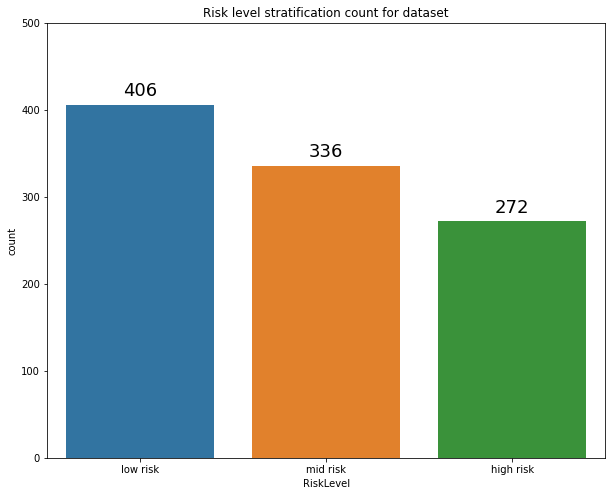
\includegraphics[scale = 0.7]{stats_risk.png}
    \caption{Risk level stratification count}
    \label{Risk_level_count}
\end{figure}

%%%%-------------------------------------------------------------------%%%%

\noindent
2) What type of benefit you might hope to get from data mining. 

\begin{itemize}
    \item Data Mining study is to solve the maternal healthcare problem, mainly for the rural areas of a developing country.
    \item Study will help to reduce the problems of pregnant women as well as a newborn baby.
    \item Thus, risk stratification using data mining will increase the safety of maternal health as well as the unborn baby
\end{itemize}

\pagebreak
%%%%-------------------------------------------------------------------%%%%
\noindent
3) Discuss data quality issues: For each attribute,\\

\noindent
a) Are there problems with the data? \\ 

None of attributes is missing in dataset, hence minimum quality issues \\

\noindent
b) What might be an appropriate response to the quality issues? \\

If quality issues existed, these can be resolved using 
\begin{itemize}
    \item If attribute data is missing for a row, dropping/discarding individual pregnant women data
    \item Filling missing dataset with most common values or mean of columns
    \end{itemize}

\noindent
(ii) Implement \\
          
(1) Decision Tree & (2) Random Forest &  (3) Naïve Bayes Classifier &
(4) KNN classifier \\

compare the performances using k-fold cross validation and other tuning techniques.

%%%%-------------------------------------------------------------------%%%%
\section{Feature Selection}

\noindent
\subsection{Chi-squared stats}
This score can be used to select the features with the highest values for the test chi-squared statistic from X, which must contain only non-negative features such as booleans or frequencies relative to the classes. \\

Chi-square test values to check whether or not a particular attribute is influential on the response reported in table \ref{chi_sq}

\begin{table}[h]
\centering
\caption{Chi-square test to get influential attributes}
\label{chi_sq}
\begin{tabular}{ccccccc}
\hline
\toprule
{} &    Age & SystolicBP & DiastolicBP &     BS & BodyTemp & HeartRate \\
\hline
\midrule
chi-square     & 500.92 &     556.24 &      323.26 & 663.13 &    61.96 &    212.91 \\
p-value        &   0.00 &       0.00 &        0.00 &   0.00 &     0.00 &      0.00 \\
Critical value & 133.48 &      58.62 &       50.89 &  83.51 &    29.14 &     50.89 \\
Influential    &    yes &        yes &         yes &    yes &      yes &       yes \\
\hline
\end{tabular}
\end{table}

\pagebreak

\noindent
\subsection{Correlation Heat Map}
\begin{figure}[h]
    \centering
    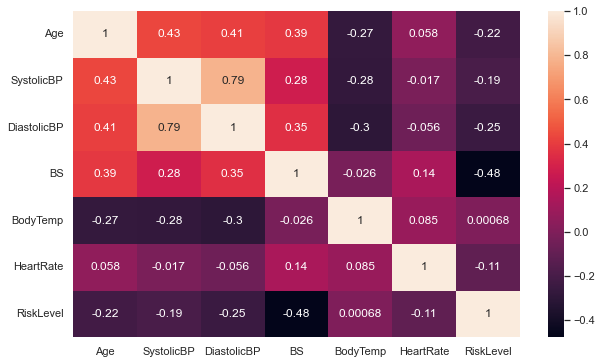
\includegraphics[scale = 0.5]{cor_heat_map.png}
    \caption{Correlation Heat Map}
    \label{corr_heat_MAp}
\end{figure}

\noindent
\begin{itemize}
    \item Blood Sugar is highly correlated with Risk Level 
    \item Diastolic BP $>$ Age $>$ Systolic BP have significant correlation with Risk Level
\end{itemize}

\noindent
\subsection{Random Forest feature importance}
\begin{figure}[h]
    \centering
    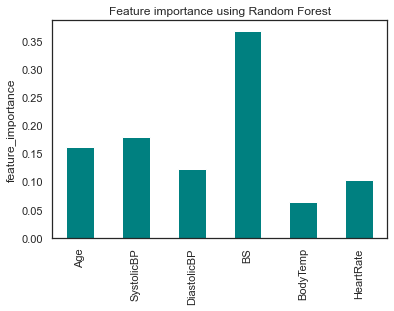
\includegraphics[scale = 0.7]{FS_imp.png}
    \caption{Feature selection using Random Forest}
    \label{FS_RF}
\end{figure}

\noindent
\begin{itemize}
    \item Blood Sugar is most importance feature using Random forest feature selection
\end{itemize}

\pagebreak

\noindent
\subsection{Coefficient importance}
\begin{figure}[h]
    \centering
    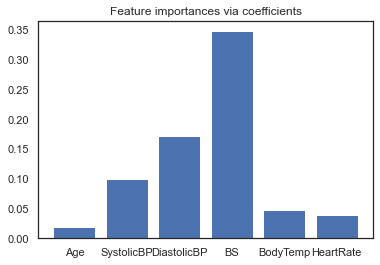
\includegraphics[scale = 0.7]{coef_imp.png}
    \caption{Feature selection using Coefficient importance}
    \label{FS_RF}
\end{figure}

\noindent
\begin{itemize}
    \item Blood Sugar is most importance feature using Random forest feature selection 
\end{itemize}


\noindent
\subsection{Mutual information classification}
\begin{figure}[h]
    \centering
    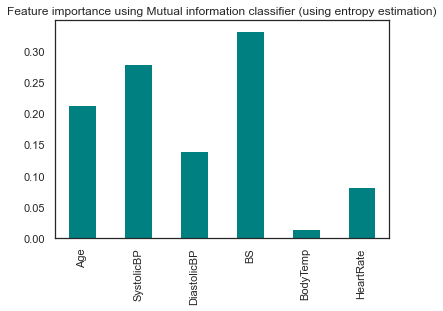
\includegraphics[scale = 0.7]{FS_entropy.png}
    \caption{Feature selection using Mutual information classification}
    \label{FS_entropy}
\end{figure}

\pagebreak

\noindent
\subsection{Recursive Feature selection using Decision Tree}
\begin{figure}[h]
    \centering
    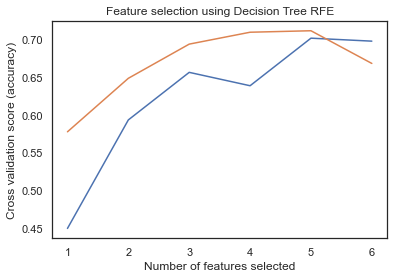
\includegraphics[scale = 0.7]{FS_Dtree.png}
    \caption{Feature selection using Decision Tree (RFE method)}
    \label{FS_entropy}
\end{figure}

\noindent
\subsection{Recursive Feature selection using SVM}
\begin{figure}[h]
    \centering
    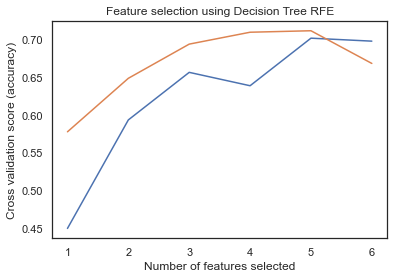
\includegraphics[scale = 0.7]{FS_Dtree.png}
    \caption{Feature selection using SVM (RFE method)}
    \label{FS_entropy}
\end{figure}

\noindent
\begin{itemize}
    \item recursive feature selection used 
    \item Both in backward and forward RFE blood sugar and Diastolic BP are important features 
    \item minimum 5 features to be selected for high accuracy, but 6 were retained as accuracy did not fall from 6th feature addition
\end{itemize}

\pagebreak
%%%%-------------------------------------------------------------------%%%%

\section{Multi-collinearity check}
\begin{figure}[h]
    \centering
    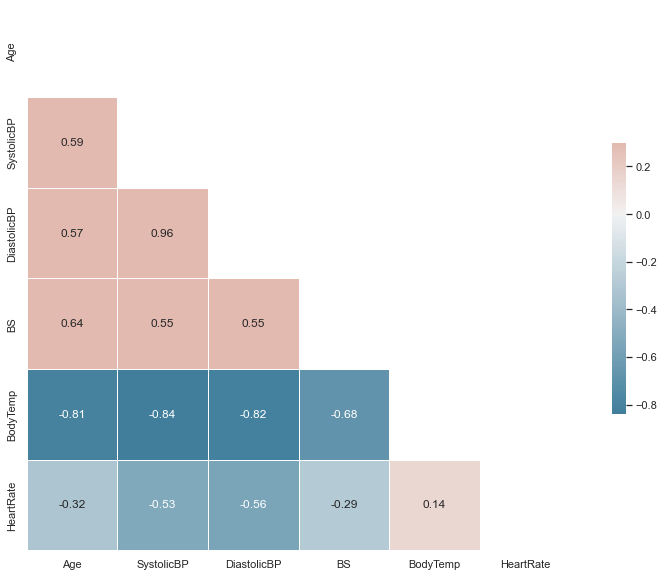
\includegraphics[scale = 0.5]{heat_mult.png}
    \caption{Checking for multicollinearity between features}
    \label{heat_mult}
\end{figure}

\begin{itemize}
    \item No perfect col-linearity observed, but correlation among attributes
\end{itemize}

\pagebreak
%%%%-------------------------------------------------------------------%%%%
\section{Classification Model implementation and Result}

\begin{table}[]
\caption{Model Performance}
\label{Model_perf}
\centering
\scalebox{1}{
\begin{tabular}{cccccc}
\hline
\toprule
& Accuracy score & Precision & Recall & F-score & ROC-AUC score \\
\hline
\midrule
Decision Tree &           0.81 &      0.81 &   0.82 &    0.81 &          0.86 \\
Random Forest &           0.82 &      0.82 &   0.82 &    0.82 &          0.87 \\
Naive Bayes &           0.50 &      0.50 &   0.48 &    0.48 &          0.61 \\
K-NN &           0.80 &      0.80 &   0.80 &    0.80 &          0.85 \\
\hline
\end{tabular}}
\end{table}

%%%%-------------------------------------------------------------------%%%%
\subsection{Decision Tree} \\ 
\begin{itemize}
    \item Decision tree is trained using entropy criterion and initially with default hyper-parameters in sklearn python library  
    \item data set is split into 70:30 ratio for training:testing 
\end{itemize}

\subsubsection{Result}
\begin{itemize}
    \item Accuracy score: 0.810 (High out of sample accuracy)
    \item Precision : 0.806 
    \item Recall : 0.817 
    \item F-score : 0.808
    \item ROC AUC of test set: 0.863 (suggests high performance)
\end{itemize}

\subsubsection{Confusion Matrix}
\begin{figure}[h]
    \centering
    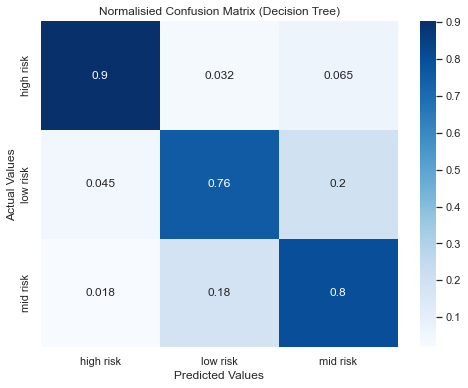
\includegraphics[scale = 0.5]{DT_CM.png}
    \caption{Normalised Confusion Matrix (Decision Tree)}
    \label{DT_CM}
\end{figure}

\pagebreak

\subsubsection{ROC AUC Curve}
\begin{figure}[h]
    \centering
    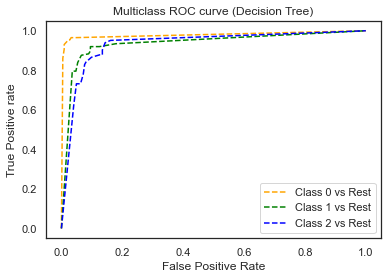
\includegraphics[scale = 0.8]{ROC_DT.png}
    \caption{ROC AUC curve (Decision Tree)}
    \label{ROC_DT}
\end{figure}

\subsubsection{Cross Validation Results}

Data was divided into 15 equal-size partitions and accuracy score of 0.85 was achieved with a standard deviation of 0.04. 

This was carried out at successively increasing height of decision tree and entropy criterion: \\

\begin{table}[h]
\centering
\caption{Result using cross validation at different height}
\label{tab:my_label}
\begin{tabular}{c|c|c}
\hline
Tree Depth & Accuracy & Std Dev. \\
\hline
\midrule
1 & 0.59 & 0.04 \\
5 & 0.70 & 0.04 \\
10 & 0.78 & 0.05 \\
15 & 0.84 & 0.04 \\
20 & 0.85 & 0.04 \\ 
\hline    
\end{tabular}
\end{table}

\pagebreak

\subsubsection{Hyper-parameter Tuning using GridSearchCV}
Data was divided into 15 equal-size partitions and this was repeated 3 times using RepeatedStratifiedKFold function for cross validation. \\

For hyper-parameter tuning, GridSearchCV is used. \\
\begin{itemize}
    \item Inputs for tuning is selection of criterion for division at node : Entropy vs Gini. 
    \item Tree depth : range between 1 and 20 
    \item Result from tuning : entropy as criterion and 19 as tree depth, but depth of 8 was selected as 0.8 accuracy was achieved at tree depth 8 and higher possiblity of overfitting at higher depth. 
    \item decision tree is plot using Graphviz with tree depth 8. 
\end{itemize}

%%%%-------------------------------------------------------------------%%%%
\subsection{Random Forest} \\ 
\begin{itemize}
    \item Random Forest is trained using 10 estimators and entropy as criterion for split. Initially with default hyper-parameters in sklearn python library  
    \item data set is split into 70:30 ratio for training:testing 
\end{itemize}

\subsubsection{Result}
\begin{itemize}
    \item Accuracy score: 0.820 (High out of sample accuracy)
    \item Precision : 0.816 
    \item Recall : 0.824 
    \item F-score : 0.817
    \item ROC AUC of test set: 0.868 (suggests high performance)
\end{itemize}

\pagebreak
\subsubsection{Confusion Matrix}
\begin{figure}[h]
    \centering
    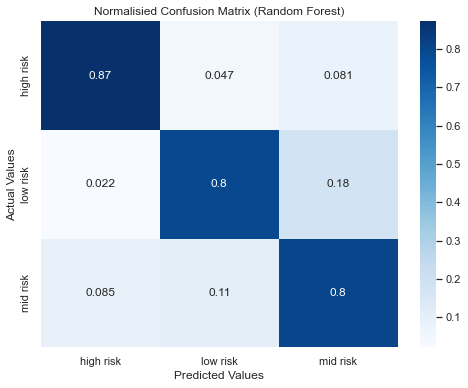
\includegraphics[scale = 0.5]{RF_CM.png}
    \caption{Normalised Confusion Matrix (Random Forest)}
    \label{RF_CM}
\end{figure}

\subsubsection{ROC AUC Curve}
\begin{figure}[h]
    \centering
    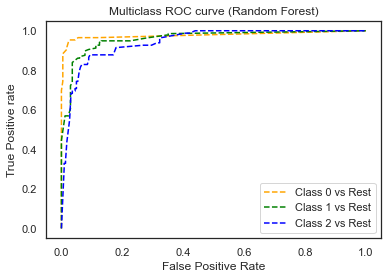
\includegraphics[scale = 0.8]{ROC_RF.png}
    \caption{ROC AUC curve (Random Forest}
    \label{ROC_DT}
\end{figure}

\pagebreak

\subsubsection{Cross Validation Results}

Data was divided into 15 equal-size partitions and accuracy score of 0.85 was achieved with a standard deviation of 0.13. 

This was carried out at successively increasing height of decision tree and entropy criterion: \\

\begin{table}[h]
\centering
\caption{Result using cross validation at different estimator size}
\label{tab:my_label}
\begin{tabular}{c|c|c}
\hline
Estimator size & Accuracy & Std Dev. \\
\hline
\midrule
1 & 0.78 & 0.04 \\
5 & 0.85 & 0.03 \\
10 & 0.85 & 0.03 \\
15 & 0.85 & 0.03 \\
20 & 0.85 & 0.03 \\ 
\hline    
\end{tabular}
\end{table}

\subsubsection{Hyper-parameter Tuning using GridSearchCV}
Data was divided into 15 equal-size partitions and this was repeated 3 times using RepeatedStratifiedKFold function for cross validation. \\

For hyper-parameter tuning, GridSearchCV is used. \\
\begin{itemize}
    \item Inputs for tuning is selection of criterion for division at node : Entropy vs Gini. 
    \item Estimator size : range between 1 and 20 
    \item Result from tuning : entropy as criterion and 20 as estimator size, but estimator size of 10 was selected as 0.85 accuracy was achieved at size 10 and higher possiblity of overfitting at higher estimator size. 
\end{itemize}
%%%%-------------------------------------------------------------------%%%%
\subsection{Naive Bayes} \\ 
\begin{itemize}
    \item Random Forest is trained with default hyper-parameters in sklearn python library  
    \item data set is split into 70:30 ratio for training:testing 
\end{itemize}

\subsubsection{Result}
\begin{itemize}
    \item Accuracy score: 0.518 (poor out of sample accuracy)
    \item Precision : 0.499 
    \item Recall : 0.480 
    \item F-score : 0.482
    \item ROC AUC of test set: 0.061 (suggests low performance)
\end{itemize}

\subsubsection{Confusion Matrix}
\begin{figure}[h]
    \centering
    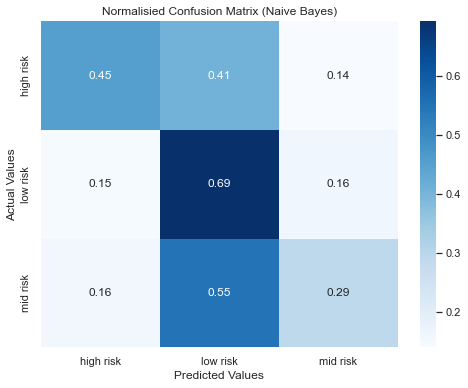
\includegraphics[scale = 0.5]{NB_CM.png}
    \caption{Normalised Confusion Matrix (Naive Bayes)}
    \label{RF_CM}
\end{figure}

\subsubsection{ROC AUC Curve}
\begin{figure}[h]
    \centering
    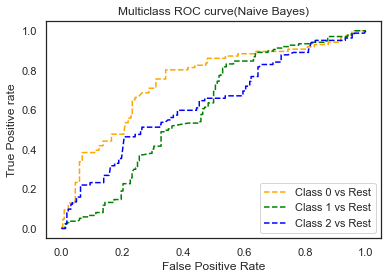
\includegraphics[scale = 0.8]{ROC_NB.png}
    \caption{ROC AUC curve (Naive Bayes}
    \label{ROC_DT}
\end{figure}

\pagebreak

\subsubsection{Cross Validation Results}

Data was divided into 15 equal-size partitions and accuracy score of 0.45 was achieved with a standard deviation of 0.10. 

This was carried out at successively increasing alpha value from 0.05 to 0.95 with increment of 0.1 at each step and fit\_prior = True : \\

\begin{table}[h]
\centering
\caption{Result using cross validation at different alpha values}
\label{tab:my_label}
\begin{tabular}{c|c|c}
\hline
Alpha & Accuracy & Std Dev. \\
\hline
\midrule
0.1 & 0.46 & 0.06 \\
0.3 & 0.46 & 0.06 \\
0.5 & 0.46 & 0.06 \\
0.7 & 0.46 & 0.06 \\
1.0 & 0.46 & 0.06 \\ 
\hline    
\end{tabular}
\end{table}

\subsubsection{Hyper-parameter Tuning using GridSearchCV}
Data was divided into 15 equal-size partitions and this was repeated 3 times using RepeatedStratifiedKFold function for cross validation. \\

For hyper-parameter tuning, GridSearchCV is used. \\
\begin{itemize}
    \item Inputs for tuning is selection of criterion for division at node : alpha in range 0 to 1. 
    \item fit prior boolean value True or False 
    \item Result from tuning : alpha = 0.45 and fit\_prior = True are best hyper-parameter 
\end{itemize}
%%%%-------------------------------------------------------------------%%%%
\subsection{K Nearest Neighbour } \\ 
\begin{itemize}
    \item KNN is trained with nearest\_neighbors = 1, metric = 'minkowski', p = 2 and with default hyper-parameters in sklearn python library  
    \item data set is split into 70:30 ratio for training:testing 
\end{itemize}

\subsubsection{Result}
\begin{itemize}
    \item Accuracy score: 0.803 (good out of sample accuracy)
    \item Precision : 0.802 
    \item Recall : 0.803 
    \item F-score : 0.803
    \item ROC AUC of test set: 0.852 (suggests high performance)
\end{itemize}

\subsubsection{Confusion Matrix}
\begin{figure}[h]
    \centering
    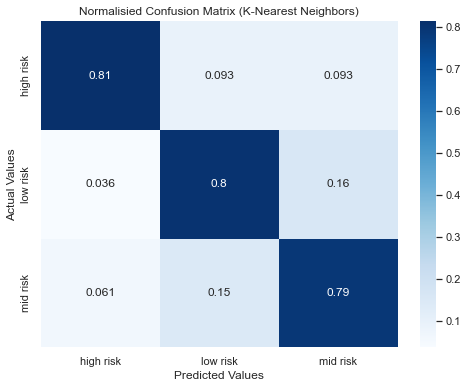
\includegraphics[scale = 0.5]{KNN_CM.png}
    \caption{Normalised Confusion Matrix (KNN)}
    \label{RF_CM}
\end{figure}

\subsubsection{ROC AUC Curve}
\begin{figure}[h]
    \centering
    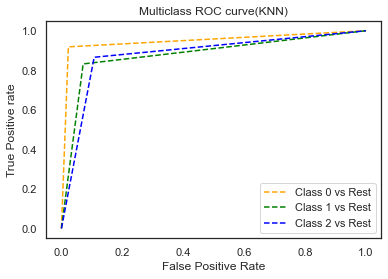
\includegraphics[scale = 0.8]{ROC_KNN.png}
    \caption{ROC AUC curve (KNN)}
    \label{ROC_DT}
\end{figure}

\pagebreak

\subsubsection{Cross Validation Results}

Data was divided into 15 equal-size partitions and accuracy score of 0.84 was achieved with a standard deviation of 0.04. 

This was carried out at successively decreasing nearest neighbour from 10 to 1 with increment of 0.1 at each step and minkowski metric is used with p = 2 which is euclidean distance : \\

\begin{table}[h]
\centering
\caption{Result using cross validation at different n\_neighbour values}
\label{tab:my_label}
\begin{tabular}{c|c|c}
\hline
n\_neighbour & Accuracy & Std Dev. \\
\hline
\midrule
10 & 0.69 & 0.05 \\
7 & 0.70 & 0.05 \\
5 & 0.71 & 0.05 \\
3 & 0.71 & 0.05 \\
1 & 0.84 & 0.04 \\ 
\hline    
\end{tabular}
\end{table}

\subsubsection{Hyper-parameter Tuning using GridSearchCV}
Data was divided into 15 equal-size partitions and this was repeated 3 times using RepeatedStratifiedKFold function for cross validation. \\

For hyper-parameter tuning, GridSearchCV is used. \\
\begin{itemize}
    \item Inputs for tuning is selection of criterion: nearest neighbour in range 1 to 10. and p value in range of 1 to 5 for minokswi distance metric  
    \item Result from tuning : nearest neighbour = 1 and p = 1 are best hyper-parameter but p = 2 was chosen as almost same accuracy 
\end{itemize}

\pagebreak
%%%%-------------------------------------------------------------------%%%%
\section{Performance of classification algorithm comparison}

\begin{figure}[h]
    \centering
    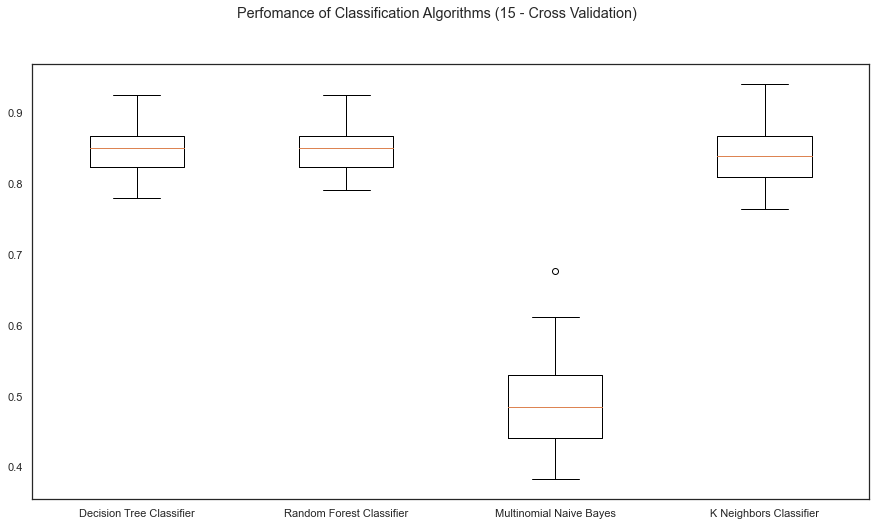
\includegraphics[scale = 0.5]{Class_perf.png}
    \caption{classification algorithm accuracy comparison using cross validation}
    \label{class_perf}
\end{figure}

\noindent
Random Forest $>$ Decision Tree $>$ KNN Classifer $>$ Multinominal Naive Bayes 

%%%%-------------------------------------------------------------------%%%%

\subsection*{Question 2}

\noindent
(a) Implement Apriori and FP-growth algorithm. Cite any sources helpful to you for implementing the algorithms. \\ 

Sol. Please refer jupyter notebook and github/gitlab repository for code. \\

\noindent
(b) Modify the algorithms to achieve the same task (preferably with some improvement). Clearly mention the difference in the modified algorithm. \\

Implementation Apriori using Hashtree is modification in aprori alogrithm for improvement. \\

Sol. Please refer jupyter notebook and github/gitlab repository for code.

%%%%-------------------------------------------------------------------%%%%


\end{document}
